\section{Introduction}

\subsection{Background}

\subsubsection{Revolve NTNU}

Revolve NTNU is a student organization dedicated to constructing electric formula cars for the international \acrfull{fs} competitions. In the course of one year, an \acrfull{ev} is designed, constructed and tested before entering multiple competitions, facing off against comparable vehicles and teams from other universities from around the world.

The combination of short development time and a team consisting of mostly new, inexperienced members makes for several interesting problems. This report will focus on a specific embedded system, the \acrfull{vcu}, and the issues encountered when developing it. As the \acrshort{ev} is almost exclusively made from custom parts, the different systems on the car depends heavily on each other. This means that changes done to the \acrshort{vcu} will invariably affect the rest of the vehicle and vice-versa. 


\subsubsection{The vehicle control unit}

The vehicle control unit is the central control system of the \acrshort{ev}. It is responsible for handling sensory data from the vehicle and the driver, and then output fitting data to the motor controllers (\emph{inverters}) for each electric motor. The \acrshort{vcu} is only allowed to send set points to the inverters when the \acrshort{ev} is in \emph{Drive-Enable mode}. Transitioning into this mode requires action from the driver.



%In addition, the \acrshort{vcu} is to
%\begin{itemize}
%    \item put the vehicle into Drive-Enable mode when certain criteria are met.
%    \item perform safety checks on inputted data and take appropriate action if errors are found.
%    \item interface with the \acrfull{ins}.
%    \item interface with the data logger provided by competition officials, as per EV 4.6 \cite{fsgrules}.
%\end{itemize}

The team member responsible for the \acrshort{vcu} is not responsible for the implementation of the control algorithms that takes vehicle and driver input and outputs motor set points. The control algorithms performs \acrfull{tv}, a technique for intelligently varying the torque on each wheel. This increases the maneuverability of the \acrshort{ev}, especially in corners. The \acrshort{vcu} is responsible for providing an environment for the control algorithms to run.

It is necessary that the VCU conforms the to \acrshort{fs} competition rules. \acrfull{fsg} is the largest competition, and their rules are considered standard \cite{fsgrules}.

% Since the vehicle is capable of speeds exceeding 110 kilometres per hour \cite{novaspeed}, the control algorithms cannot use more time than necessary. As the deadlines the \acrshort{vcu} has to uphold are critical for the survival of the vehicle and possibly the driver, it is per definition a \emph{hard real-time embedded system}. However, the exact deadline is unknown. The rule of thumb used by members is that the control loop has to run in at no lower than 100 \si{\hertz}. {\color{red}(Should really find some data on this.)}


\subsubsection{Analysis of 2019 system}\label{sec:2019sys}

The \acrshort{ev} made by Revolve NTNU during the 2019 season is called Nova. A simple overview of the systems and their interractions can be seen in figure \ref{fig:vcu19_system}.

In the 2019 season, Revolve NTNU made their newest \acrshort{ev}, Nova. (see figure \ref{fig:nova}).

%\begin{figure}[H]
%    \centering
%    \includegraphics[width=\textwidth]{media/Nova.png}
%    \caption{Revolve NTNU 2019's electric vehicle, Nova.}
%    \label{fig:nova}
%\end{figure}

\begin{figure}[H]
    \centering
    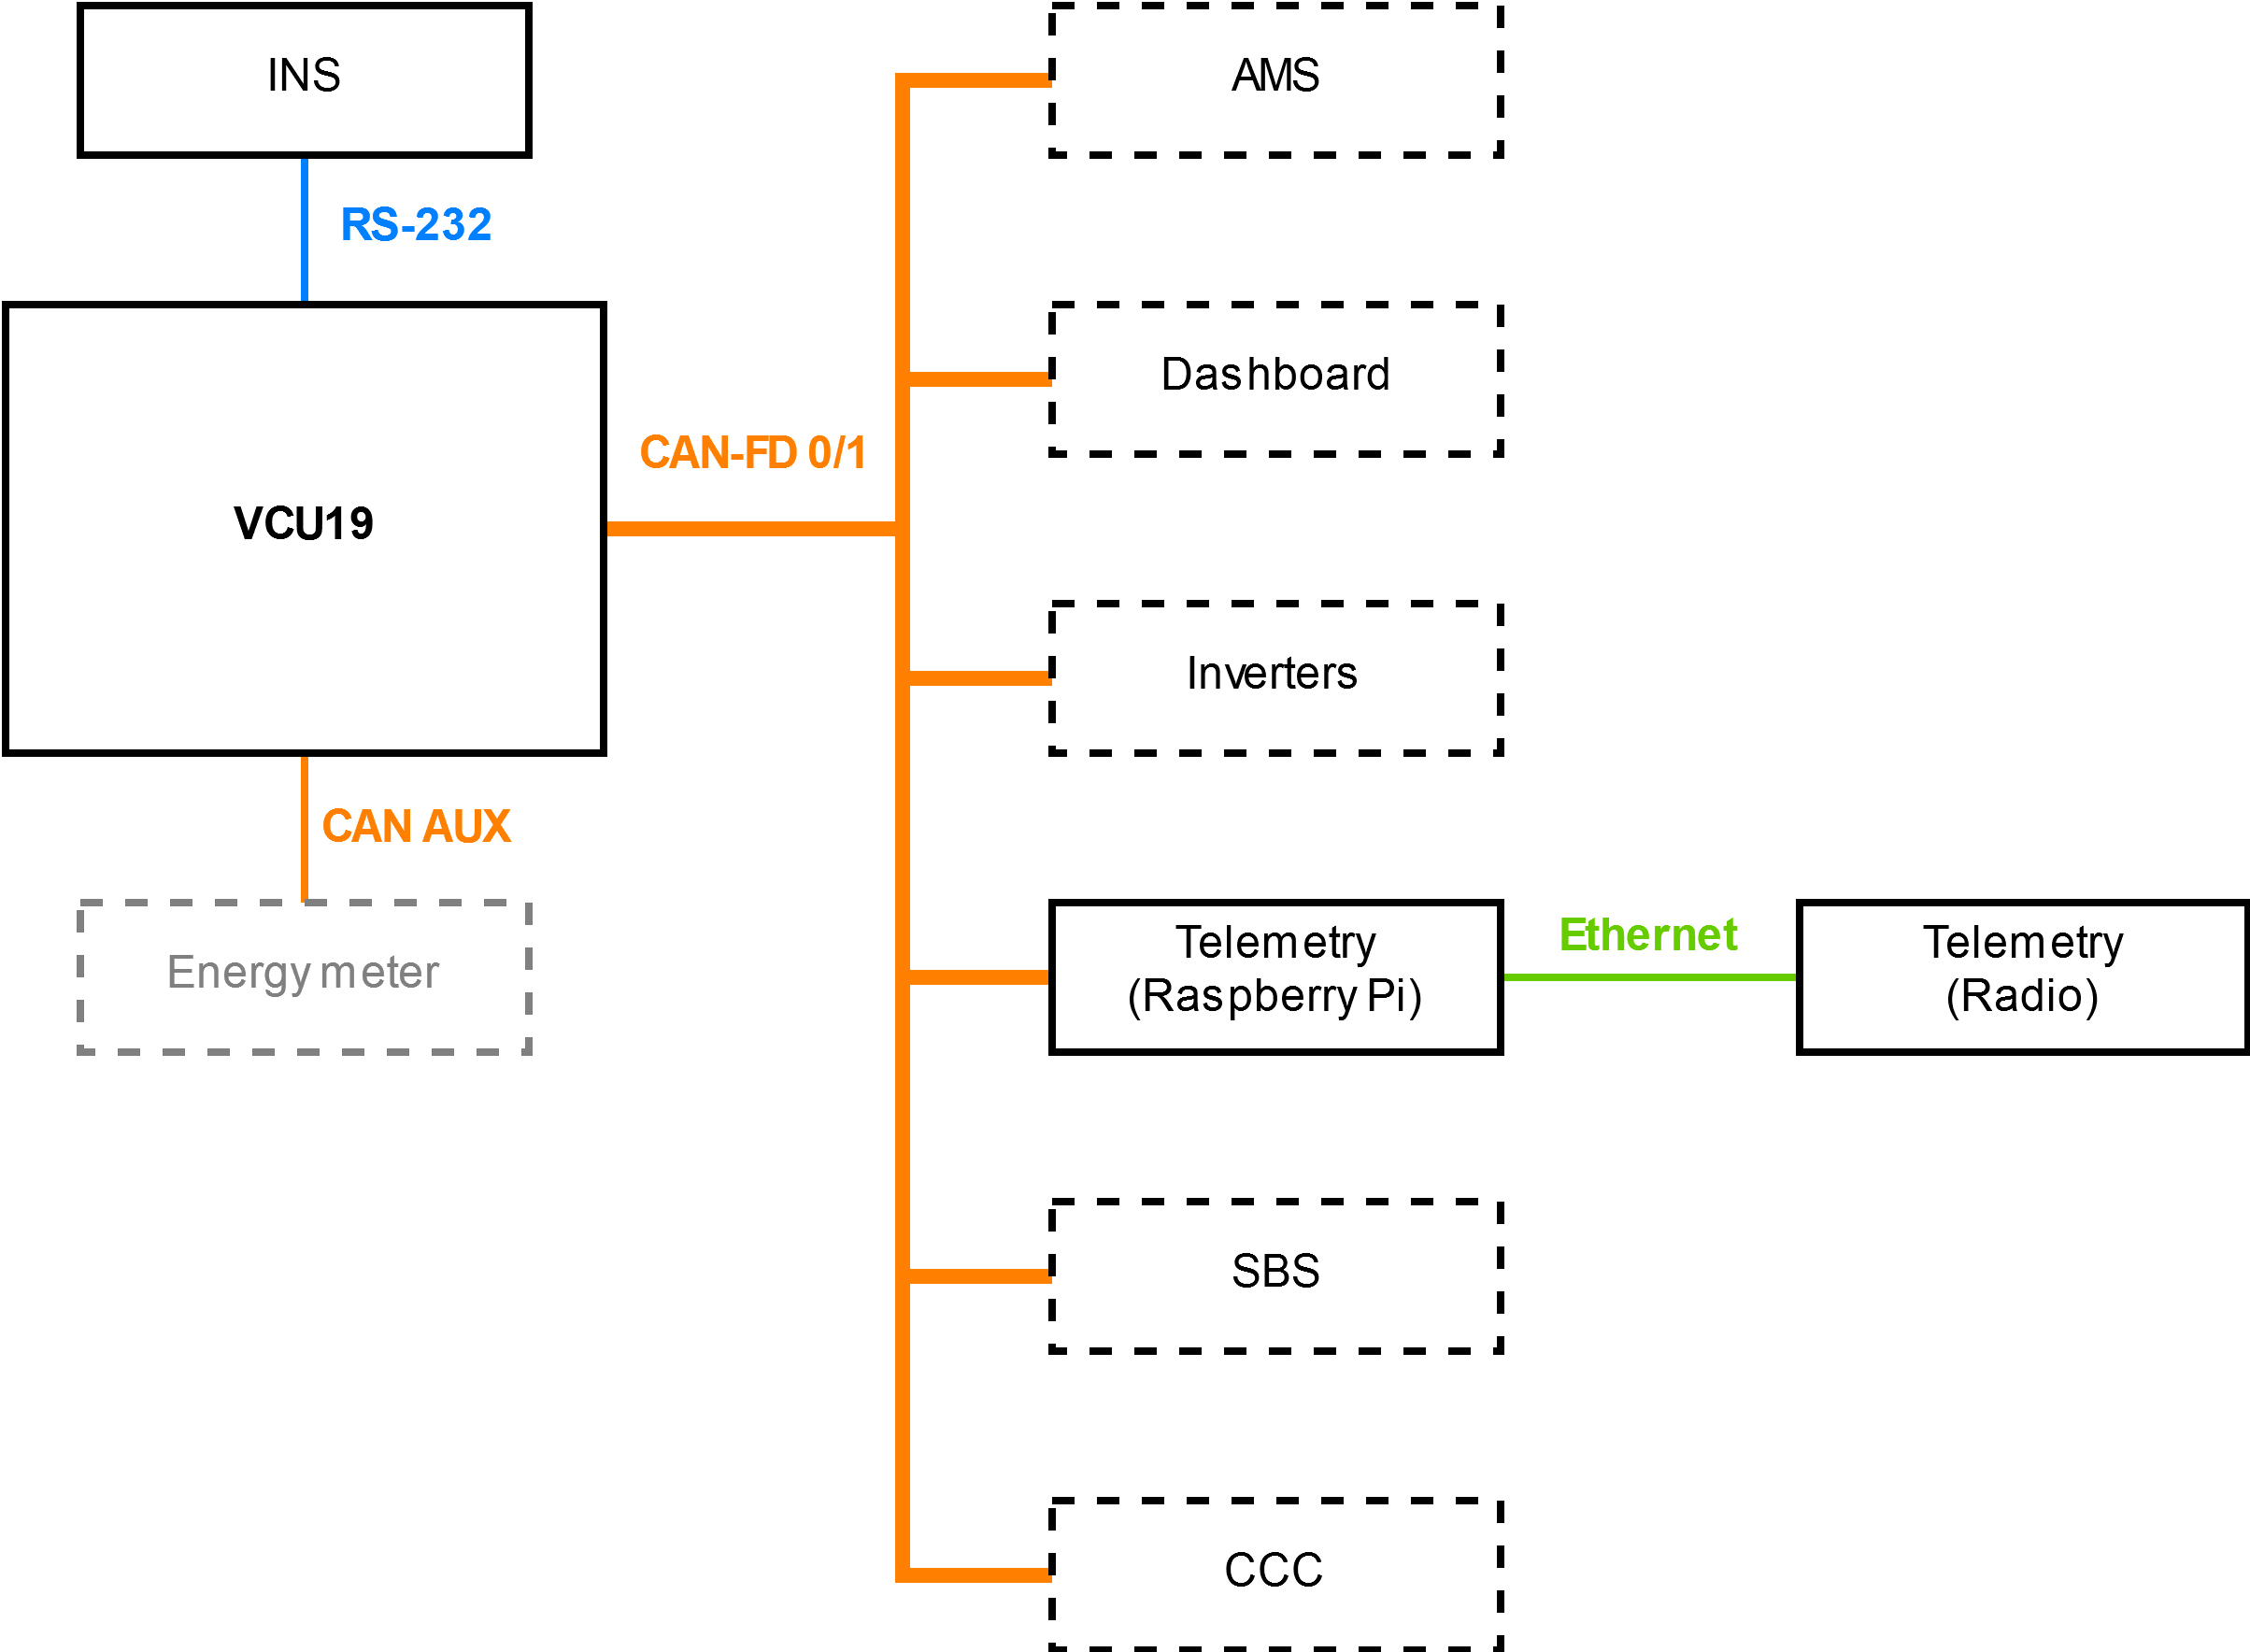
\includegraphics[width=.85\textwidth]{media/vcu19_system.png}
    \caption{Author's rendition of embedded system structure in Nova. Systems developed by other team members have dotted borders.}
    \label{fig:vcu19_system}
\end{figure}

To fulfill the requirements of the \acrshort{tv} control algortihm, \acrfull{vcu19} was designed around a new processing platform, the Xilinx Zynq-7000 \cite{zynq}. It is a \acrfull{soc} with a dual core ARM Cortex A9 processor and embedded \acrfull{fpga}. 

Advanced processing units like the Zynq-7000 are typically only available in \acrfull{bga} packages, meaning packages with all pins placed in a grid pattern on the bottom. This makes assembly and debugging harder, a serious concern considering the rapid development methodologies necessary in Revolve NTNU. A 3D render of \acrshort{vcu19} can be seen in figure \ref{fig:vcu19}.

\begin{figure}[H]
    \centering
    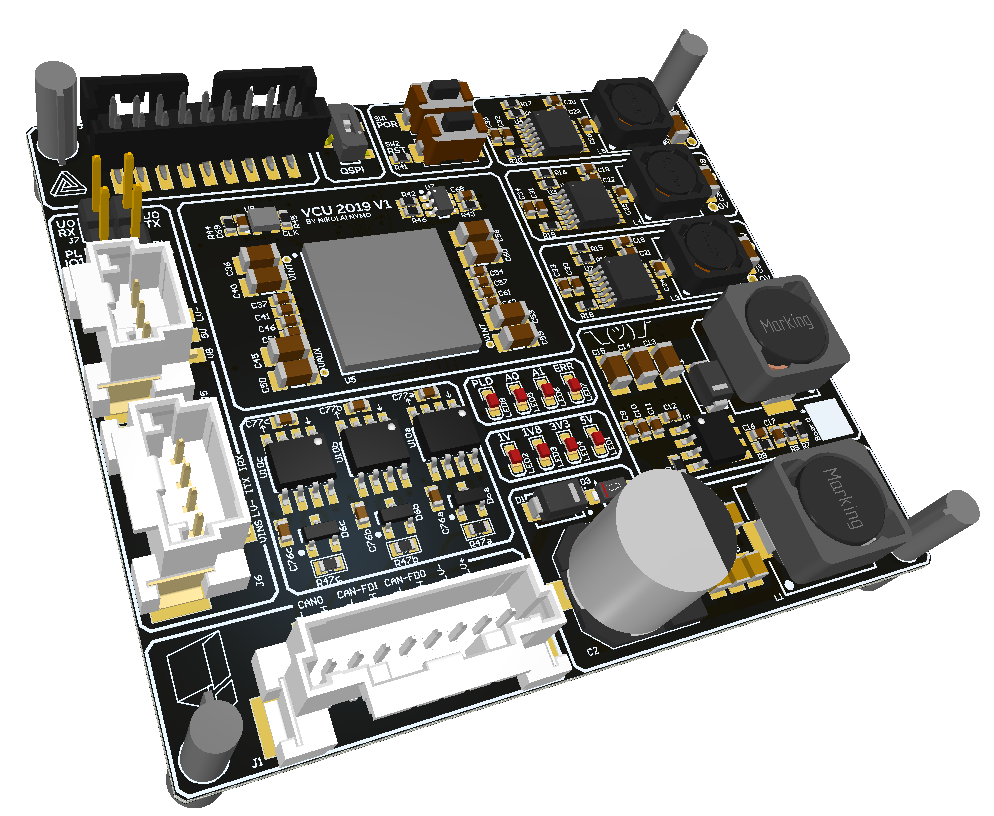
\includegraphics[width=.95\textwidth]{media/vcu19.png}
    \caption{\acrshort{vcu} from 2019 season. It was designed by team member Nikolai Nymo, VCU responsible in 2019.}
    \label{fig:vcu19}
\end{figure}

Another issue encountered was the high load on the \acrfull{canfd} buses. Much of the work in Revolve NTNU is directed at analyzing data from the \acrshort{ev}. The data is transmitted from the vehicle to a base station nearby using a proprietary wireless communication system from Radionor AS \cite{radionor}. This is called the \emph{telemetry} system.

The radio must be used through an Ethernet interface and there are no other embedded systems on the \acrshort{ev} equipped with Ethernet. This was solved by connecting a Raspberry Pi \cite{rpi} to the two \acrshort{canfd} buses of the car using two PCAN-FD USB dongles \cite{pcan}. The Raspberry Pi is equipped with an Ethernet jack, allowing it to gather data from the \acrshort{canfd} buses and transmit it to the radio.

This solution introduces two issues. Firstly, this means that all the data that are to be sent over telemetry has to be present on the buses. As a result, the buses operate at nearly maximum capacity, introducing the risk of bus congestion (i.e. loss of messages).

The other issue is that the telemetry translation adds weight to the \acrshort{ev}. The accumulated weight of the Raspberry Pi and the two dongles amounts to almost 200\si{\gram}. Revolve NTNU works hard to reduce the weight of the vehicle as it increases the possible acceleration and allows for shorter lap times.


\subsection{Scope}

This report covers the design, assembly and testing of \acrfull{vcu20}. The new design reduces the hardware complexity of the system (while keeping the performant Zynq-7000 \acrshort{soc} platform) and reduces both total vehicle weight and \acrshort{canfd} bus load. 

%In addition we will take a closer look at the CAN-FD buses connecting the embedded systems on the vehicle.



%\subsection{Interfacing systems}

%The VCU gathers data from other embedded systems on the car. First and foremost we talk about the sonsor broadcasting system (SBS) and the inertial navigation system (INS). 
%\subsubsection{SBS}

%The SBS consists of two equal embedded systems, one placed in the front of the vehicle and one placed in the rear of the vehicle. These boards samples sensor data from and around the wheel and motor assemblies. The SBS's are both connected to the two CAN-FD buses running through the vehicle.

%\subsubsection{INS}

%The INS is an off-the-shelf solution, more precisely a VectorNav VN-300 Rugged. It uses two GPS antennaes, one on the front and one on the main hoop behind the driver, to determine the position, heading, speed and acceleration of the vehicle. The INS has two independent serial interfaces, interface 1 operating on RS-232 voltage levels, and interface 2 operating on TTL voltage levels. The only difference between the two interfaces in terms of functionality is that firmware update of the INS is available through interface 1 only. 

%This, in addition to the higher voltage used on interface 1 making it more resistant to noise, is the reason VCU19 communicated with the INS over interface 1. Note that this requires a TTL to RS-232 level shifter circuit on the VCU.

%\subsubsection{Inverters}

%The inverters converts the DC voltage from the high voltage batteries to a three-phase AC which can be used to drive the electric motors. This is by far the most complex embedded system on the vehicle. It consists of two controller cards, each controlling two inverter power cards. This makes for a total of four motor inverters, one for each motor. The inverter control cards are connected to the two CAN-FD buses, accepting messages containing \emph{set points} for the inverters, meaning how fast each motor shall turn.

%\subsubsection{Telemetry}

%The telemetry system on the vehicle is a long range radio transciever that allows for communication and monitoring of the car from a base station. The radio system is a RadioNor CRE2-144-LW which utilises phase-shift arrays to transmit signals reliably over long distances. The radio interfaces with the vehicle through an Ethernet port, receiving and transmitting UDP packages. In 2019, no other embedded system on the car used Ethernet, and a Respberry Pi 3 B+ was connected to the CAN-FD buses with two PCAN-FD USB dongles so that the embedded systems could interface with the telemetry.

%\subsubsection{Torque vectoring}

%Torque vectoring is the software system that takes the current state of the car and translates this to a desired torque on each of the four motors. It allows for better vehicle handling, especially in turns. It is a software system which should run on the VCU, but the code itself is developed and maintained by another team member. It is therefore crucial that the VCU is capable of running the TV regulation loop at a certain frequency and can supply the required resources (memory and storage). Research shows that the TV control loop has to run at 100Hz minimum to be effective.
 


